Em um sistema de refrigeração, há vários processos operados por vários maquinários, equipamentos e válvulas. Um desses equipamentos é o compressor que tem a função de receber um determinado gás a baixa temperatura e pressão e aumentar a pressão e, consequentemente, a temperatura. Esse processo pode ser esquematizado pela figura abaixo, onde o compressor está indicado pelo círculo amarelo.
\begin{figure}[!htbp]
	  \centering
	  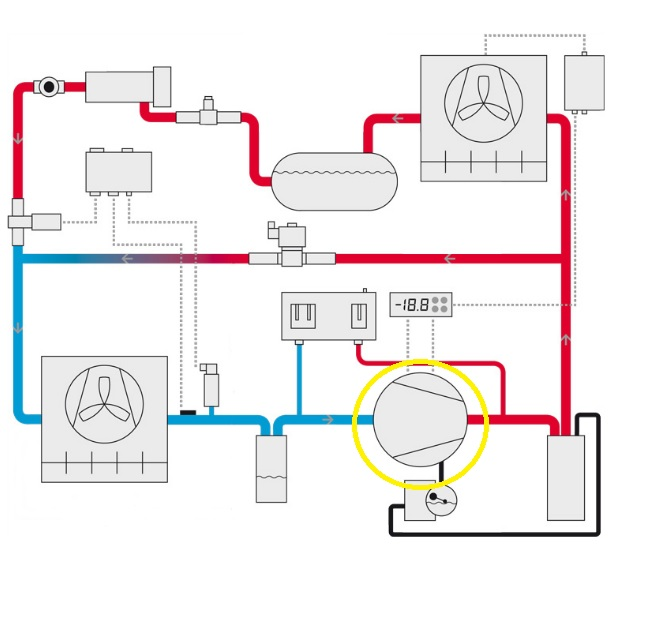
\includegraphics[scale=0.7]{editaveis/figuras/compressor}
	  \caption[Esquematização processo refrigeração]{Esquematização de um processo de refrigeração. O compressor se localiza no circulo amarelo.\footnotemark}
	  \label{compressor}
	\end{figure}
	\footnotetext{Fonte:Emerson Technologies}
	\FloatBarrier
Analisando como base a turbina WMS1000 Wind Turbine da Eolewater, percebe-se que dentre os inúmeros tipos de compressores existentes, o compressor do tipo espiral (Scroll Compressor) é o melhor e mais recomendado, principalmente pela sua capacidade de operação  e pelo seu tamanho reduzido, que é essencial visto que o espaço é muito limitado dentro turbina. Ele também pode ser combinado com outros compressores para dar ao sistema uma maior eficiência e capacidade\cite{compressors}.

Após a escolha do tipo de compressor, deve-se analisar entre os vários tipos de configuração de um compressor espiral pode ter e escolher um que adeque aos requisitos do projeto. Tomando como base a WMS1000, um compressor de aproximadamente 15KW  deverá ser usado em duplicidade para o sistema de refrigeração. 

A empresa escolhida para ser a fornecedora desse compressor foi a Emerson Electric Company, que tem tradição e tecnologia de ponta nessa área. Será usada a série de compressores Copeland Scroll™.  Essa escolha foi feita através da análise das características de cada modelo dado pela empresa como mostra a foto abaixo. Como a expectativa era de que o compressor tivesse uma potência de 15KW, e não dispondo desse modelo na empresa, foi escolhido o modelo digital ZBD 76KCE-TFD, que tem um pequeno acréscimo de potência, tornando-o o mais adequado. 

\textit{Copeland Scroll Digital Model Overview}

	\begin{figure}[!htbp]
	  \centering
	  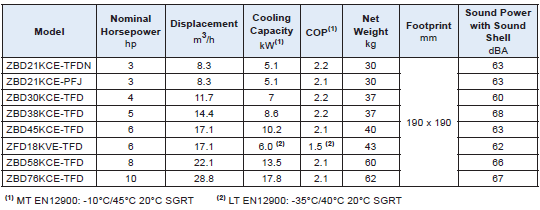
\includegraphics[scale=0.5]{editaveis/figuras/tabela_compressores}
	  \caption[Modelos de compressores]{Tabela com modelos de compressores da EmersonTM e suas características principais.\footnotemark}
	  \label{tabela_compressores}
	\end{figure}
	\footnotetext{Fonte:Emerson Technologies}
	\FloatBarrier
A EmersonTM disponibiliza seus compressores com vários tipos de líquidos refrigerantes, mais deve-se trabalhar com os materiais que possam ter o mínimo de impacto negativo na natureza. 


	\begin{figure}[!htbp]
	  \centering
	  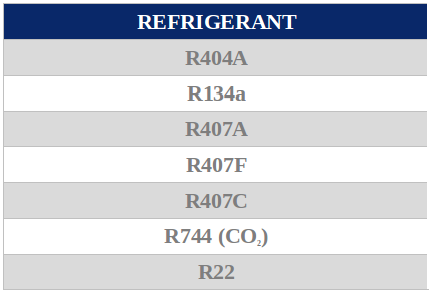
\includegraphics[scale=0.4]{editaveis/figuras/tabela_gases_refrigerantes}
	  \caption[Gases refrigerantes]{Gases refrigerantes disponibilizados pela Emerson em seus compressores.\footnotemark}
	  \label{gases_compressores}
	\end{figure}
	\footnotetext{Fonte:Emerson Technologies}
\FloatBarrier
Analisando os tipos de refrigerantes, o melhor que se poderia usar, levando em consideração seus impactos ambientais, seria o R-410A. O R-410A é um gás com efeito inofensivo a camada de ozônio, mais não ao aquecimento global \cite{essencials_r410A}. Como a EmersonTM não disponibiliza tal gás refrigerante, a escolha mais apropriada será o R-407C, que é  um substituto do R-22, um gás largamente usado e de alto impacto na camada de ozônio e no aquecimento global \cite{epa2014}. 

O R-407C vem sendo utilizado na substituição do R-22, pois o R-410A não pode ser o substituo do R-22 por causa do alto nível de pressão em que trabalha os compressores \cite{epa2014}. Mas a EmersonTM não disponibiliza o R-407C para o modelo selecionado de compressor, por isso, decidiu-se utilizar o R-407A no compressor do projeto, ainda assegurando um requisito ambiental e operacional. 

Assim, para o líquido refrigerante R407-A, o compressor espiral de modulação terá as seguintes características gerias de operação: 

	\begin{figure}[!htbp]
	  \centering
	  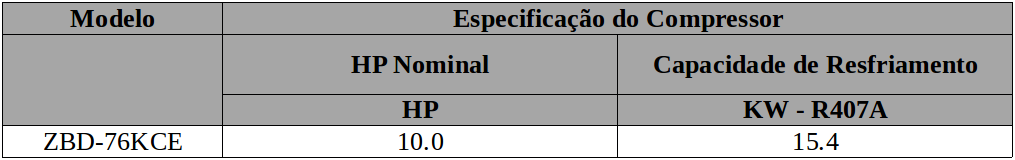
\includegraphics[scale=0.4]{editaveis/figuras/tabela_especificacao_compressor}
	  \caption[Especificação Compressor]{Características gerais do compressor.\footnotemark}
	  \label{gases_compressores}
	\end{figure}
	\footnotetext{Fonte:Emerson Technologies}
	\FloatBarrier
Abaixo segue várias informações do fabricante sobre o Compressor modelo ZBD-76KCE:

	\begin{itemize}
	 \item Características Gerais:
	 
	\begin{figure}[!htbp]
	  \centering
	  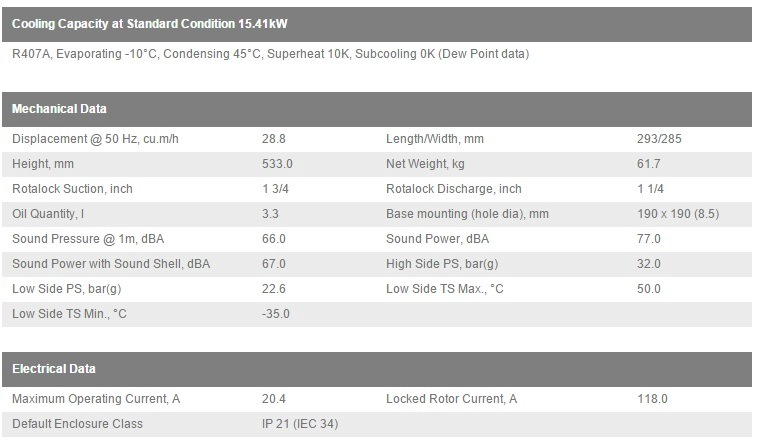
\includegraphics[scale=0.7]{editaveis/figuras/tabela_cooling_capacity}
	  \caption[Capacidade de cooling]{Características gerais do compressor.\footnotemark}
	  \label{tabela_cooling_capacity}
	\end{figure}
	\footnotetext{Fonte:Emerson Technologies}	   
	 \FloatBarrier
	 \item Envelope de Operação:  
	 
	\begin{figure}[!htbp] 
	  \centering
	  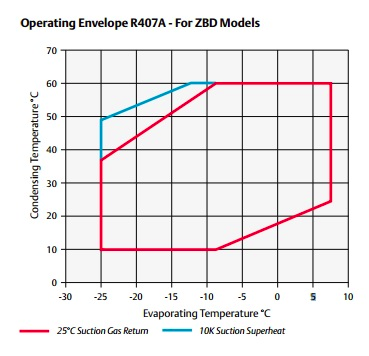
\includegraphics[scale=0.6]{editaveis/figuras/grafico_opereting_envelope}
	  \caption[Envelope de operação]{Envelope de operação.\footnotemark}
	  \label{grafico_opereting_envelope}
	\end{figure}	
	\footnotetext{Fonte:Emerson Technologies}   
	\FloatBarrier
	 \item Dimensões: 
	 
	\begin{figure}[!htbp] 
	 \centering
	  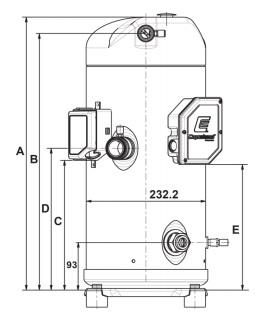
\includegraphics[scale=0.7]{editaveis/figuras/dimensao_compressor}
	  \caption[Dimensões]{Dimensões\footnotemark}
	  \label{grafico_opereting_envelope}
	\end{figure}	   
	\footnotetext{Fonte:Emerson Technologies}
	\FloatBarrier
	\begin{figure}[!htbp]
	 \centering
	  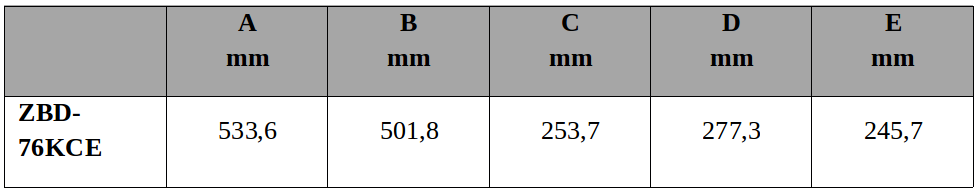
\includegraphics[scale=0.4]{editaveis/figuras/dimensao_compressor_2}
	  \caption[Dimensão compressor]{Dimensões\footnotemark}
	  \label{grafico_opereting_envelope}
	\end{figure}	   
	\footnotetext{Fonte:Emerson Technologies}
	\FloatBarrier
	\end{itemize}	